\documentclass{beamer}

\usetheme{Hannover}
\usecolortheme{dove}

\usepackage{mhchem}
\usepackage{graphicx}
\usepackage{helvet}
\usepackage{url}

\usepackage[german]{babel}
\usepackage[T1]{fontenc}
\usepackage[utf8]{inputenc}

\DeclareGraphicsRule{.tif}{png}{.png}{`convert #1 `dirname #1`/`basename #1 .tif`.png}

\title{Amine}
\author{Leon Handreke}
\date{20. April 2010}

\begin{document}

\frame{\titlepage}

\frame{\tableofcontents}

\section{Definition}
\frame
{
  \frametitle{Definition}
  \begin{quote}
    Amine sind organische Abkömmlinge (Derivate) des Ammoniaks (NH3), bei dem ein oder mehrere Wasserstoffatome durch Alkyl- oder Arylgruppen ersetzt sind.
  \end{quote}
  \small{Wikipedia}
}

\section{Überblick über die Amine}
\subsection{Typen}
\frame{
  \frametitle{Typen von Aminen}
  \begin{itemize}
  \item primäre, sekundäre, tertiäre, (quartäre)
  \item Anzahl der Substituenten
  \item Beispiel: \ce{CH3NH2}
  \end{itemize}
}

\subsection{Chemische Eigenschaften}
\frame{
  \frametitle{Chemische Eigenschaften}
  \begin{itemize}
  \item Ethylamin noch bei Raumtemperatur gasförmig, alle größeren anderen flüssig
  \item Gute Wasserlöslichkeit, da hohe Polariät
  \item Wasserstoffbrückenbindungen bei prim. und sekundären Aminen
  \item Reagiert basisch, Basenstärke nimmt mit Anzahl der Substituenten zu
  \item Ammoniakhafter Geruch
  \end{itemize}
}

\section{Methylamin}

\frame{
  \frametitle{Methylamin}
  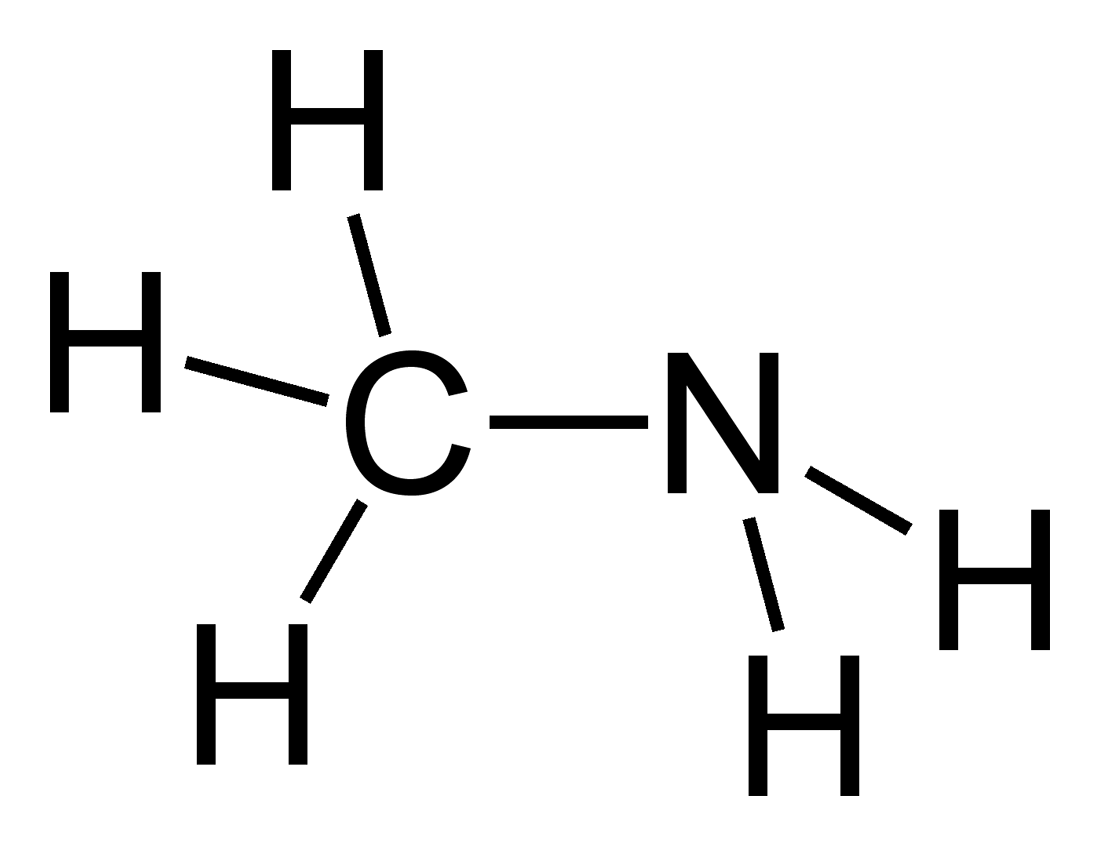
\includegraphics[width=\textwidth]{methylamin.png}
}

\subsection{Herstellung}
\frame{
  \frametitle{Herstellung}
  \begin{itemize}
  \item Umsetzung von Methanol und Ammoniak zu Methylamin und Wasser
  \item Temperaturen um $400\,^{\circ}\mathrm{C}$ nötig
  \item Nebenprodukte: Di- und Trimethylamin
  \end{itemize}
}

\frame{
  \frametitle{Reaktionsgeichung}
  \begin{center}
    \ce{CH3OH + NH3 -> CH3NH2 + H2O}
  \end{center}
}

\subsection{Eigenschaften}
\frame{
  \frametitle{Eigenschaften}
  \begin{itemize}
  \item Farbloses Gas
  \item Brennbar
  \item Reagiert in Wasser basisch
  \end{itemize}
}

\subsection{Verwendung}
\frame{
  \frametitle{Verwendung}
  \begin{itemize}
  \item Hauptsächlich Zwischenprodukt
  \item Folgeprodukte: Lösungsmittel, Farbstoffe, Pharmazeutika
  \end{itemize}
}

\section{Diazotierung}

\subsection{Diazoniumsalze}
\frame{
  \frametitle{Diazoniumsalze}
  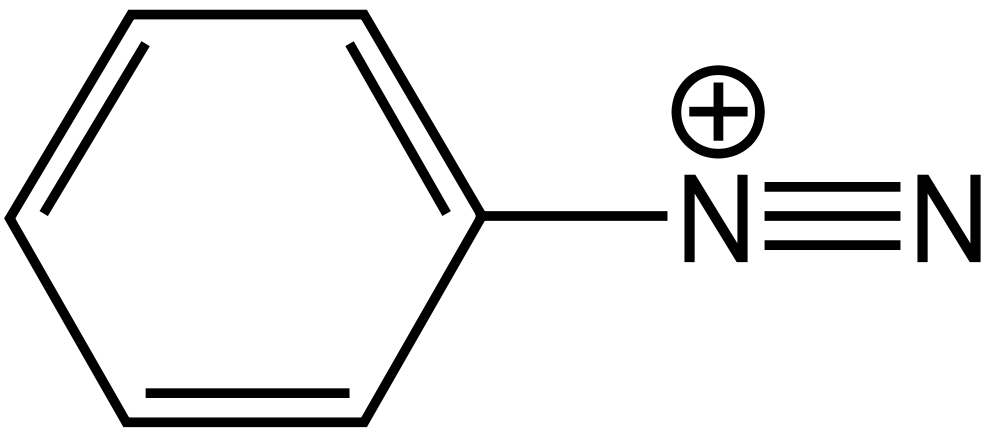
\includegraphics[width=\textwidth]{diazonium.png}
}

\frame{
  \frametitle{Diazoniumsalze - unsere Freunde?}
  \begin{itemize}
  \item Instabil
  \item Explosiv
  \item Krebserregend
  \end{itemize}
}

\subsection{Mechanismus}
\frame{
  \framtitle{Diazotierung}
  \begin{itemize}
  \item Ausgangsstoffe: primäre aromatische Amine (z.B. Anilin)
  \item Verwendung: Herstellung vom Azofarbmitteln
  \end{itemize}
}

\frame{
  \frametitle{Diazotierung}
  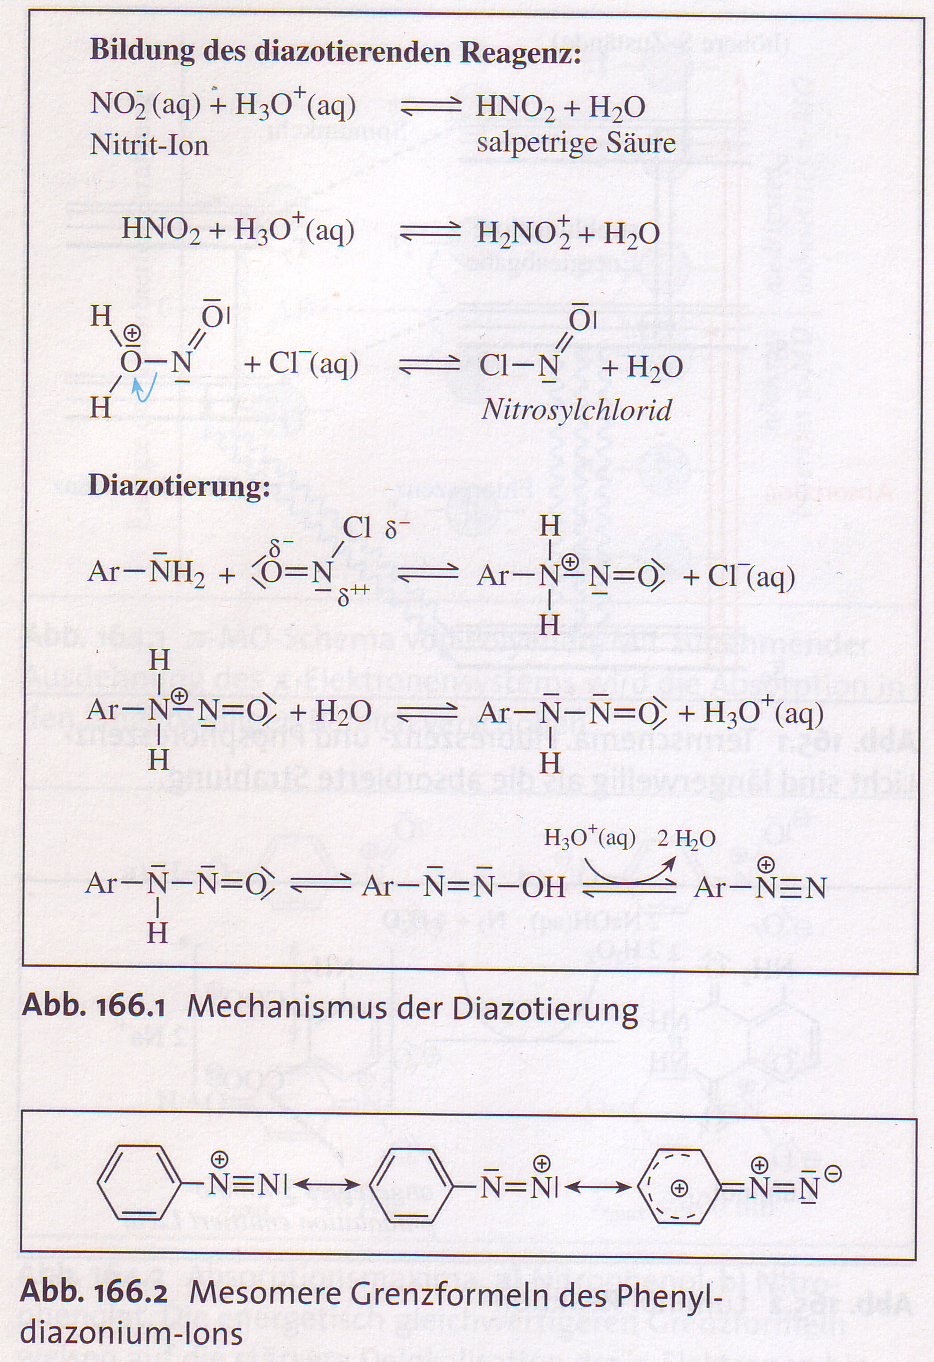
\includegraphics[width=5cm]{diazotierung.png}
}

\frame{
  \frametitle{Diazotierung}
  \begin{itemize}
  \item \ce{ArNH2 + HNO2 + HX -> [ArN2]+X- + 2H2O}
  \end{itemize}
}

\section{Polyamide}
\subsection{Eigenschaften und Verwendung}

\frame{
  \frametitle{Polyamide}
  \begin{itemize}
  \item thermoplastische Kunststoffe
  \item schmelzbar
  \item oft als Kunstfasern verwendet
  \end{itemize}
}

\subsection{Bildung}
\frame{
  \frametitle{Polyamid}
  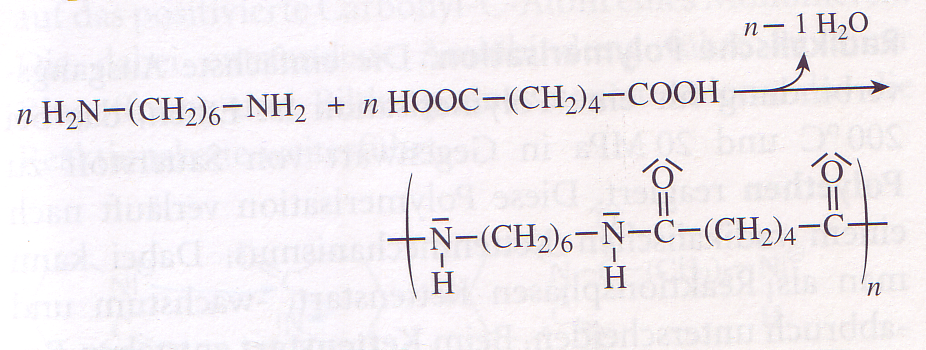
\includegraphics[width=\textwidth]{polyamid-reaktion.png}
}

\subsection{Struktur}
\frame{
  \frametitle{Polyamide}
  \begin{center}
    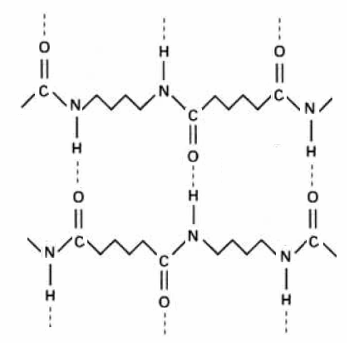
\includegraphics[width=5cm]{polyamid.png}
  \end{center}
}

\section{Quellen}
\frame{
  \frametitle{Quellen}
  \begin{itemize}
  \item \url{http://www2.chemie.uni-erlangen.de/projects/vsc/chemie-mediziner-neu/funktgruppen/amine_bc.html}
  \item \url{http://www.chemie.fu-berlin.de/chemistry/kunststoffe/amid.htm}
  \item \url{http://de.wikipedia.org/}
  \item \url{http://commons.wikimedia.org} (Illustrationen)
  \end{itemize}
}

\frame{
  \begin{center}
    \Huge{Fragen?}
  \end{center}
}
\end{document}
